This appendix presents the comprehensive component-level profiling visualizations across all 16 evaluated architectural pipeline configurations on both the academic multi-hop benchmark (\mbox{MuSiQue}) and the closed enterprise production corpus. These detailed distributions complement the summary metric tables and trade-off frontiers presented in Chapter~\ref{sec:results}.

\subsection{Component-Wise Latency Breakdowns}
\label{subsec:appendix_latency_breakdowns}

Figure~\ref{fig:latency_breakdown_combined} details the empirical execution latency decomposed across fine-grained pipeline stages: dense vector retrieval, cross-encoder neural re-ranking ($M_2$), prompt caching prefix initialization and reuse ($M_3$), query classification routing ($M_4$), and generative token synthesis across both evaluation benchmarks.

\begin{figure}[!htbp]
\centering
\begin{subfigure}{\linewidth}
  \centering
  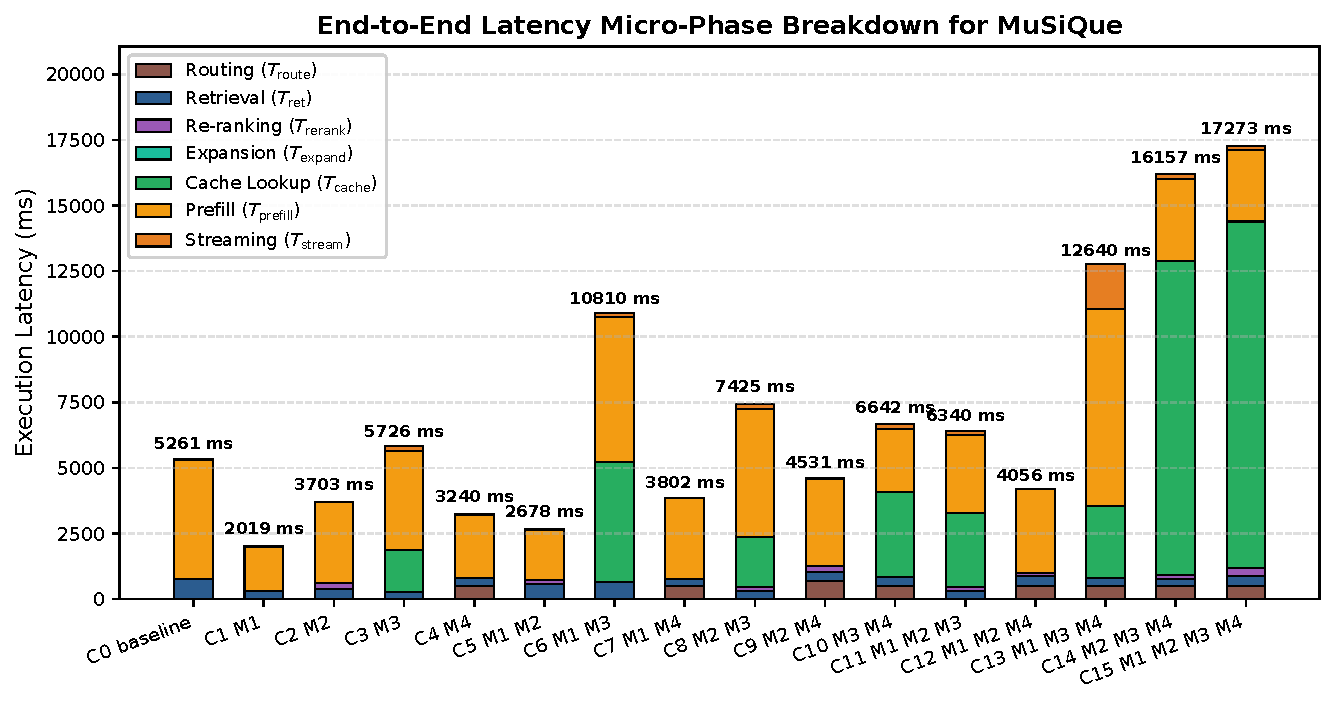
\includegraphics[width=0.88\linewidth]{figures/musique/latency_breakdown_musique.pdf}
  \caption{Academic multi-hop benchmark (MuSiQue)}
  \label{fig:latency_breakdown_musique}
\end{subfigure}
\\[0.5ex]
\begin{subfigure}{\linewidth}
  \centering
  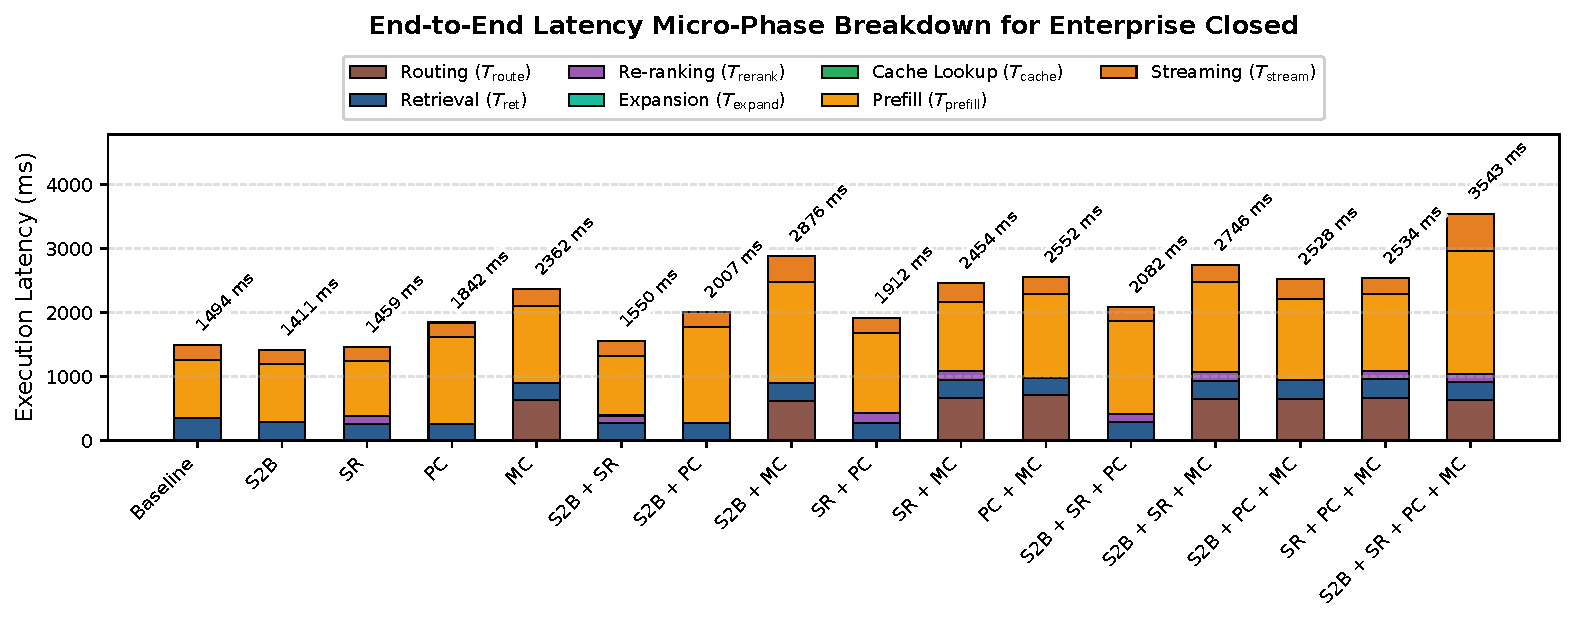
\includegraphics[width=0.88\linewidth]{figures/enterprise_closed/latency_breakdown_enterprise_closed.pdf}
  \caption{Enterprise closed benchmark corpus}
  \label{fig:latency_breakdown_enterprise}
\end{subfigure}
\caption[Component-wise execution latency breakdown across configurations]{Component-wise execution latency breakdown across all 16 pipeline configurations on (a) MuSiQue and (b) Enterprise Closed, decomposing latency across retrieval, re-ranking, prompt caching, model routing, and token generation phases. Stacked bars represent sample mean execution durations across queries, complementary to the median ($P_{50}$) profiles reported in Chapter~\ref{sec:results}.}
\label{fig:latency_breakdown_combined}
\end{figure}

\clearpage

\subsection{Operational Expenditure Component Decompositions}
\label{subsec:appendix_cost_breakdowns}

Figure~\ref{fig:cost_breakdown_combined} presents the component-wise monetary operational expenditure per 1,000 queries, isolating costs incurred from uncached context prompt tokens, context cache read lookups, generative completion tokens, auxiliary cross-encoder neural re-ranking calls, and router model classifications across both benchmark environments.

\begin{figure}[!htbp]
\centering
\begin{subfigure}{\linewidth}
  \centering
  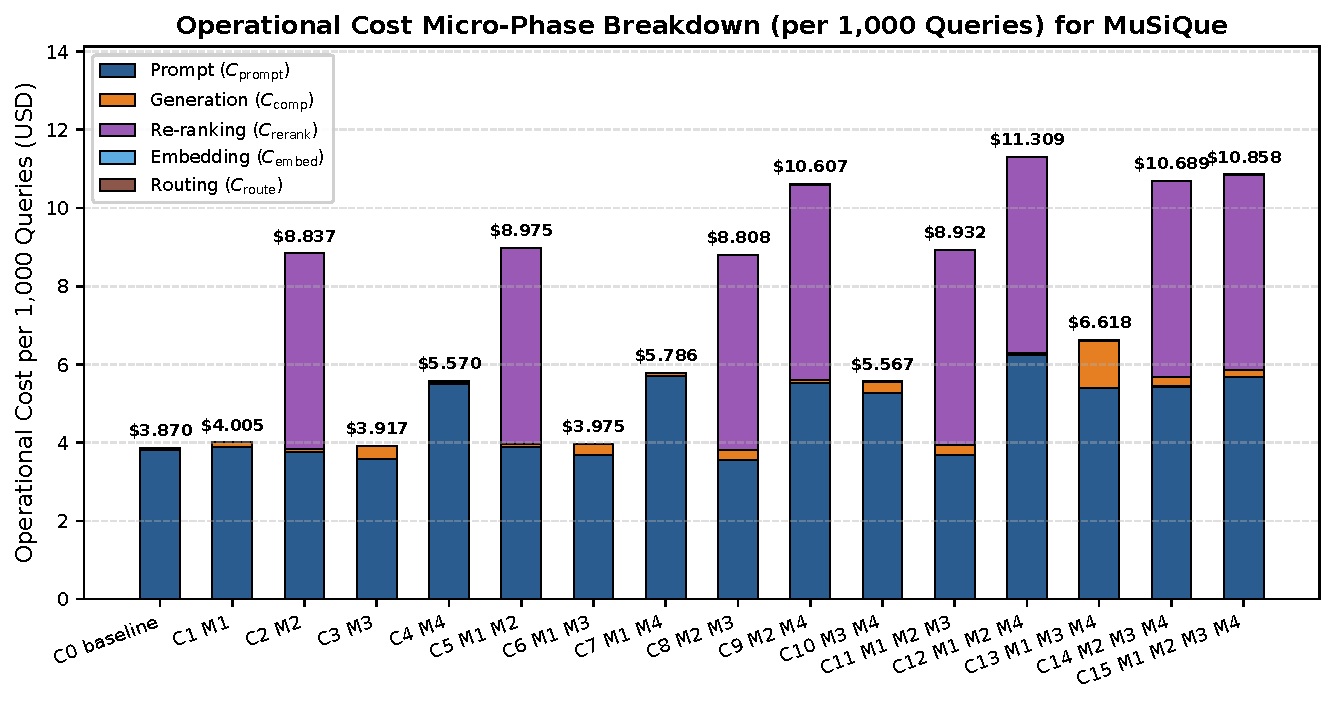
\includegraphics[width=0.94\linewidth]{figures/musique/cost_breakdown_musique.pdf}
  \caption{Academic multi-hop benchmark (MuSiQue)}
  \label{fig:cost_breakdown_musique}
\end{subfigure}
\\[0.5ex]
\begin{subfigure}{\linewidth}
  \centering
  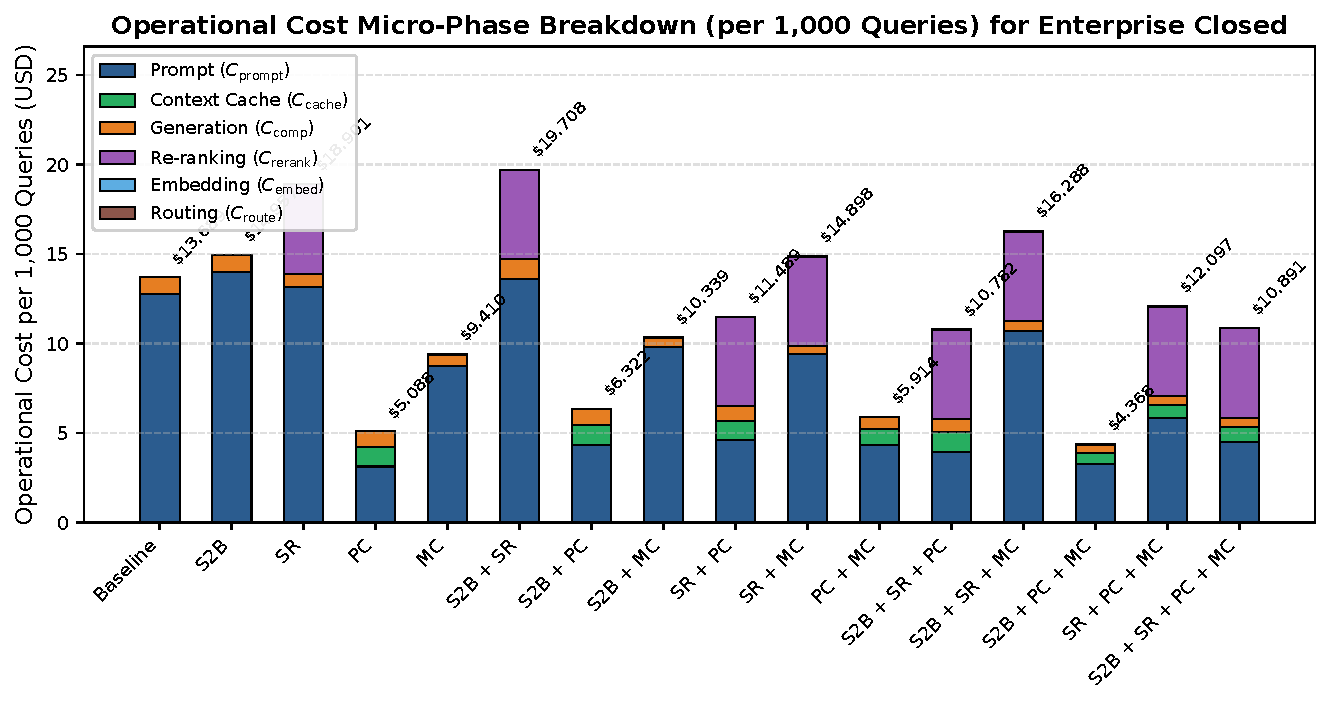
\includegraphics[width=0.94\linewidth]{figures/enterprise_closed/cost_breakdown_enterprise_closed.pdf}
  \caption{Enterprise closed benchmark corpus}
  \label{fig:cost_breakdown_enterprise}
\end{subfigure}
\caption[Component-wise operational expenditure breakdown across configurations]{Component-wise operational expenditure breakdown per 1,000 queries across all 16 pipeline configurations on (a) MuSiQue and (b) Enterprise Closed, decomposing monetary expenditure across prompt prefill, context cache lookups, generative completion, auxiliary neural re-ranking, and model routing.}
\label{fig:cost_breakdown_combined}
\end{figure}

\clearpage

\subsection{Multi-Dimensional Quality Metric Profiles}
\label{subsec:appendix_quality_lollipops}

Figure~\ref{fig:quality_lollipop_musique} and Figure~\ref{fig:quality_lollipop_enterprise} illustrate configuration-level response quality profiles across Context Precision, Context Recall, Faithfulness, and Answer Relevancy across architectural tiers ($k=0 \dots 4$).

\begin{figure}[!htbp]
\centering
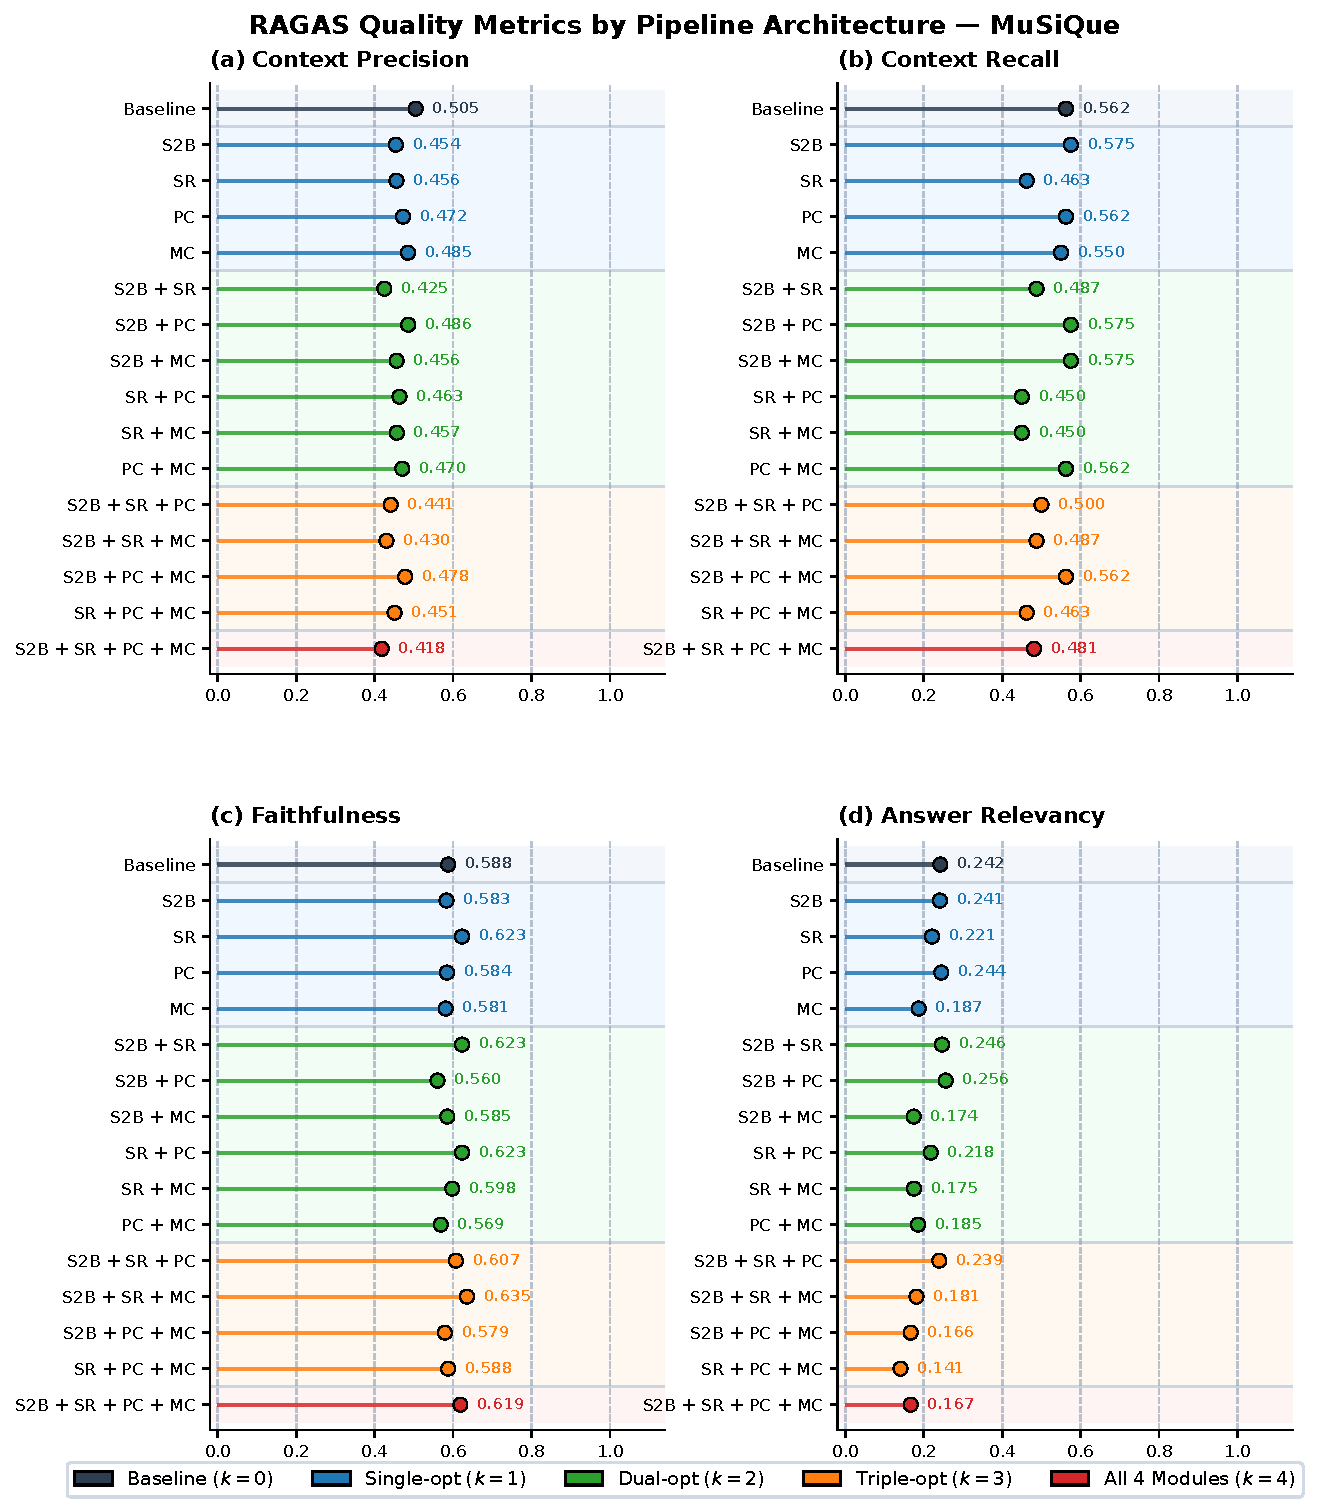
\includegraphics[width=\linewidth]{figures/musique/quality_lollipop_musique.pdf}
\caption[Multi-dimensional response quality profiles on MuSiQue]{Multi-dimensional response quality profiles across architectural configurations on the academic multi-hop benchmark (MuSiQue), comparing Context Precision, Context Recall, Faithfulness, and Answer Relevancy across architectural tiers ($k=0 \dots 4$). Horizontal lollipop plots with tier-stratified background shading isolate configuration-level variations across retrieval and synthesis dimensions.}
\label{fig:quality_lollipop_musique}
\end{figure}

\begin{figure}[!htbp]
\centering
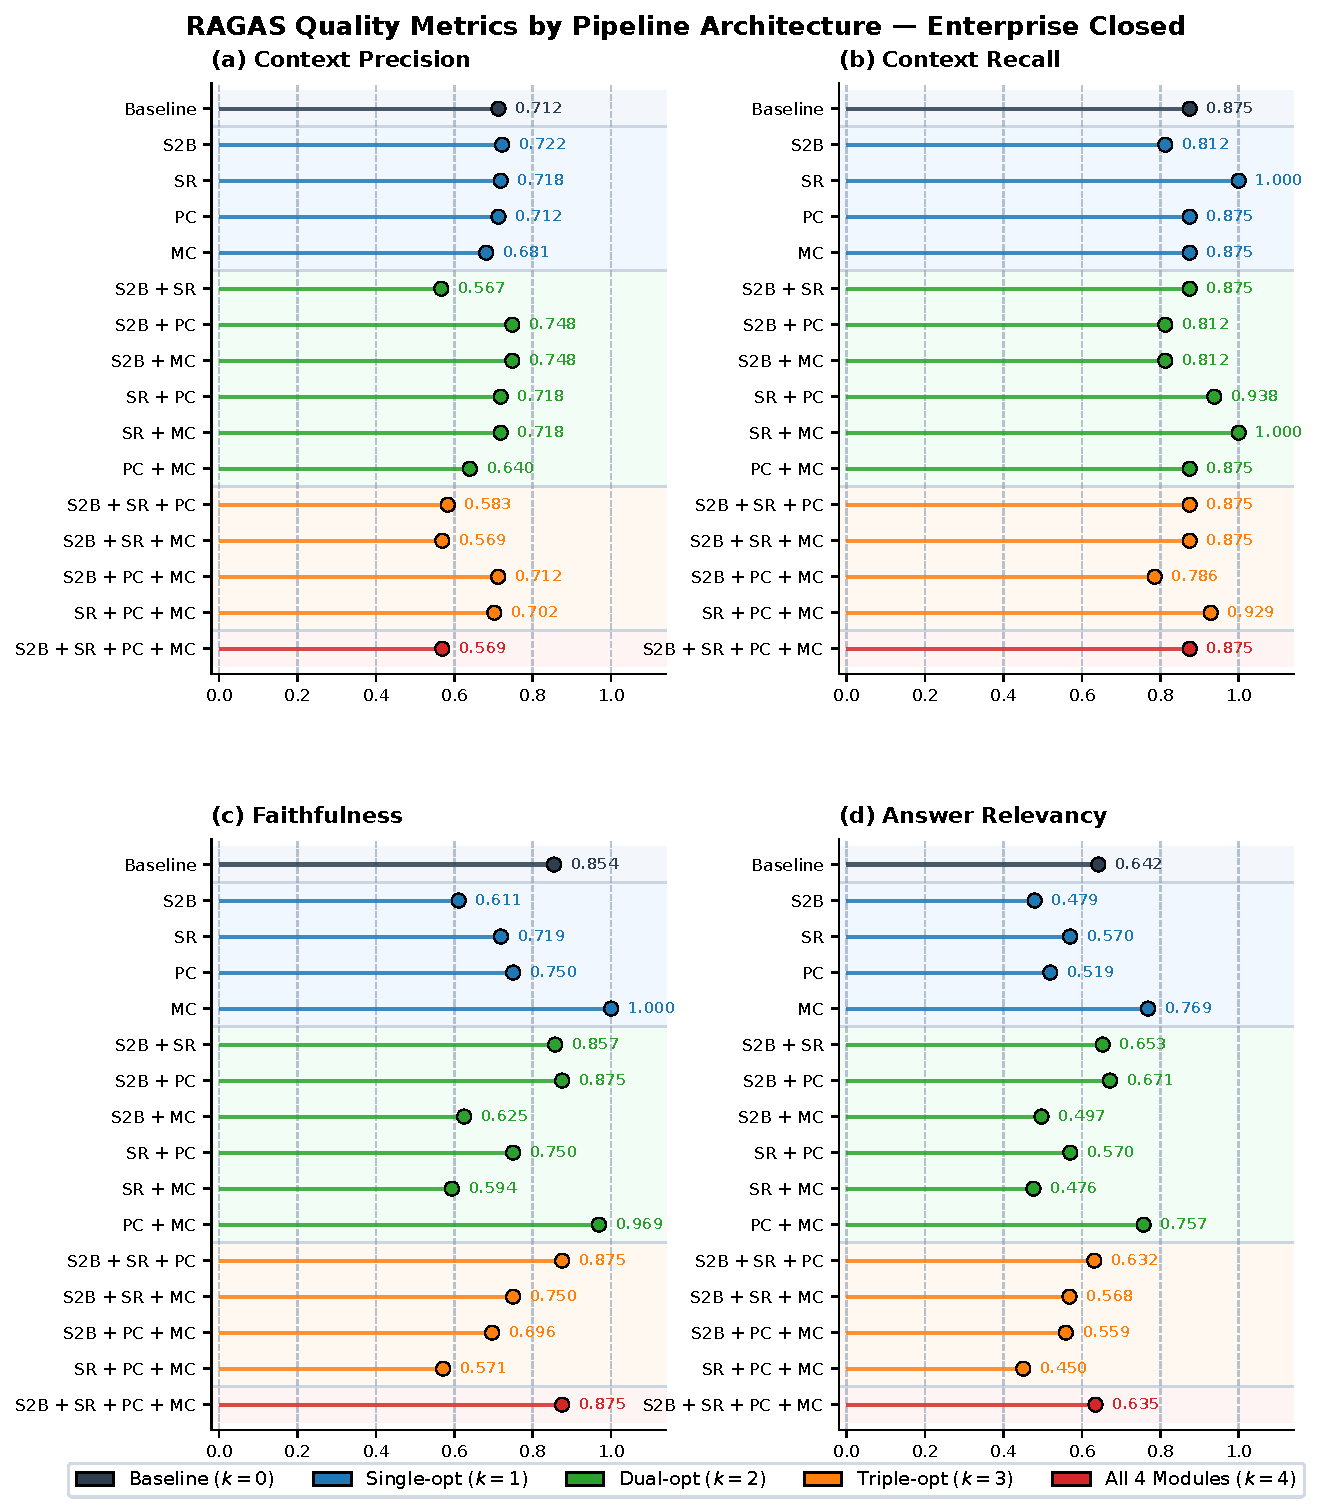
\includegraphics[width=\linewidth]{figures/enterprise_closed/quality_lollipop_enterprise_closed.pdf}
\caption[Multi-dimensional response quality profiles on Enterprise Closed]{Multi-dimensional response quality profiles across architectural configurations on the enterprise closed benchmark corpus, comparing Context Precision, Context Recall, Faithfulness, and Answer Relevancy across architectural tiers ($k=0 \dots 4$). Horizontal lollipop plots with tier-stratified background shading isolate configuration-level variations across retrieval and synthesis dimensions.}
\label{fig:quality_lollipop_enterprise}
\end{figure}
